


\tikzset{every picture/.style={line width=0.75pt}} %set default line width to 0.75pt        

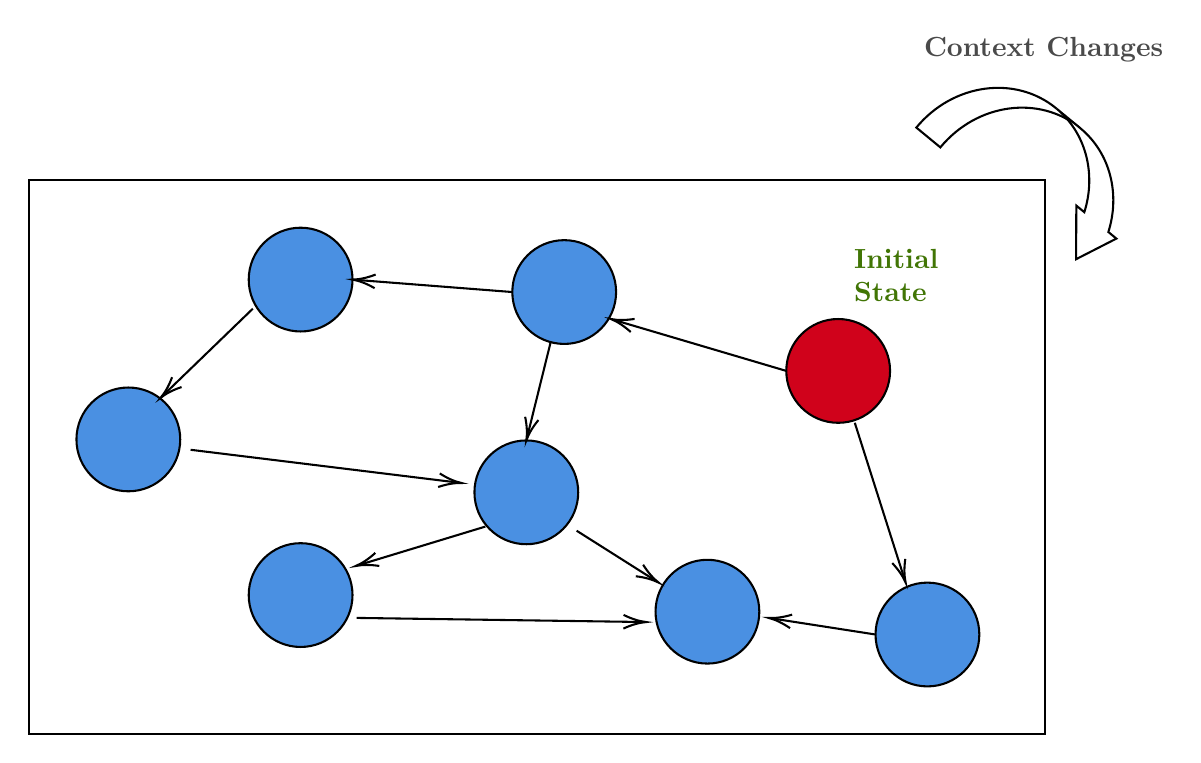
\begin{tikzpicture}[x=0.75pt,y=0.75pt,yscale=-1,xscale=1]
%uncomment if require: \path (0,410); %set diagram left start at 0, and has height of 410

%Shape: Circle [id:dp968464533790854] 
\draw  [fill={rgb, 255:red, 74; green, 144; blue, 226 }  ,fill opacity=1 ] (86,252) .. controls (86,238.19) and (97.19,227) .. (111,227) .. controls (124.81,227) and (136,238.19) .. (136,252) .. controls (136,265.81) and (124.81,277) .. (111,277) .. controls (97.19,277) and (86,265.81) .. (86,252) -- cycle ;
%Shape: Circle [id:dp21079560716947265] 
\draw  [fill={rgb, 255:red, 74; green, 144; blue, 226 }  ,fill opacity=1 ] (169,175) .. controls (169,161.19) and (180.19,150) .. (194,150) .. controls (207.81,150) and (219,161.19) .. (219,175) .. controls (219,188.81) and (207.81,200) .. (194,200) .. controls (180.19,200) and (169,188.81) .. (169,175) -- cycle ;
%Shape: Circle [id:dp5696445214135205] 
\draw  [fill={rgb, 255:red, 74; green, 144; blue, 226 }  ,fill opacity=1 ] (277.75,277.5) .. controls (277.75,263.69) and (288.94,252.5) .. (302.75,252.5) .. controls (316.56,252.5) and (327.75,263.69) .. (327.75,277.5) .. controls (327.75,291.31) and (316.56,302.5) .. (302.75,302.5) .. controls (288.94,302.5) and (277.75,291.31) .. (277.75,277.5) -- cycle ;
%Shape: Circle [id:dp5455636995208739] 
\draw  [fill={rgb, 255:red, 74; green, 144; blue, 226 }  ,fill opacity=1 ] (296,181) .. controls (296,167.19) and (307.19,156) .. (321,156) .. controls (334.81,156) and (346,167.19) .. (346,181) .. controls (346,194.81) and (334.81,206) .. (321,206) .. controls (307.19,206) and (296,194.81) .. (296,181) -- cycle ;
%Shape: Circle [id:dp8552239767397927] 
\draw  [fill={rgb, 255:red, 74; green, 144; blue, 226 }  ,fill opacity=1 ] (365,335) .. controls (365,321.19) and (376.19,310) .. (390,310) .. controls (403.81,310) and (415,321.19) .. (415,335) .. controls (415,348.81) and (403.81,360) .. (390,360) .. controls (376.19,360) and (365,348.81) .. (365,335) -- cycle ;
%Shape: Circle [id:dp49191057165067265] 
\draw  [fill={rgb, 255:red, 74; green, 144; blue, 226 }  ,fill opacity=1 ] (169,327) .. controls (169,313.19) and (180.19,302) .. (194,302) .. controls (207.81,302) and (219,313.19) .. (219,327) .. controls (219,340.81) and (207.81,352) .. (194,352) .. controls (180.19,352) and (169,340.81) .. (169,327) -- cycle ;
%Shape: Circle [id:dp20608492254875044] 
\draw  [fill={rgb, 255:red, 208; green, 2; blue, 27 }  ,fill opacity=1 ] (428,219) .. controls (428,205.19) and (439.19,194) .. (453,194) .. controls (466.81,194) and (478,205.19) .. (478,219) .. controls (478,232.81) and (466.81,244) .. (453,244) .. controls (439.19,244) and (428,232.81) .. (428,219) -- cycle ;
%Shape: Circle [id:dp40553529103941544] 
\draw  [fill={rgb, 255:red, 74; green, 144; blue, 226 }  ,fill opacity=1 ] (471,346) .. controls (471,332.19) and (482.19,321) .. (496,321) .. controls (509.81,321) and (521,332.19) .. (521,346) .. controls (521,359.81) and (509.81,371) .. (496,371) .. controls (482.19,371) and (471,359.81) .. (471,346) -- cycle ;
%Shape: Rectangle [id:dp38120662974853003] 
\draw   (63,127) -- (552.5,127) -- (552.5,394) -- (63,394) -- cycle ;
%Curve Right Arrow [id:dp7533641321758576] 
\draw  [fill={rgb, 255:red, 255; green, 255; blue, 255 }  ,fill opacity=1 ] (569.61,102.03) .. controls (549.95,85.84) and (519.78,89.99) .. (502.23,111.3) -- (490.65,101.76) .. controls (508.21,80.45) and (538.38,76.3) .. (558.04,92.49) ;\draw  [fill={rgb, 255:red, 255; green, 255; blue, 255 }  ,fill opacity=1 ] (558.04,92.49) .. controls (572.63,104.52) and (577.33,124.37) .. (571.59,142.53) -- (567.73,139.35) -- (567.63,165.17) -- (587.03,155.25) -- (583.17,152.07) .. controls (588.91,133.91) and (584.21,114.05) .. (569.61,102.03)(558.04,92.49) -- (569.61,102.03) ;
%Straight Lines [id:da45116496903786085] 
\draw    (428,219) -- (345.42,194.57) ;
\draw [shift={(343.5,194)}, rotate = 376.48] [color={rgb, 255:red, 0; green, 0; blue, 0 }  ][line width=0.75]    (10.93,-3.29) .. controls (6.95,-1.4) and (3.31,-0.3) .. (0,0) .. controls (3.31,0.3) and (6.95,1.4) .. (10.93,3.29)   ;

%Straight Lines [id:da8381673912380784] 
\draw    (461,244) -- (484.89,319.09) ;
\draw [shift={(485.5,321)}, rotate = 252.35] [color={rgb, 255:red, 0; green, 0; blue, 0 }  ][line width=0.75]    (10.93,-3.29) .. controls (6.95,-1.4) and (3.31,-0.3) .. (0,0) .. controls (3.31,0.3) and (6.95,1.4) .. (10.93,3.29)   ;

%Straight Lines [id:da23750816212213466] 
\draw    (314.5,205) -- (303.23,250.56) ;
\draw [shift={(302.75,252.5)}, rotate = 283.89] [color={rgb, 255:red, 0; green, 0; blue, 0 }  ][line width=0.75]    (10.93,-3.29) .. controls (6.95,-1.4) and (3.31,-0.3) .. (0,0) .. controls (3.31,0.3) and (6.95,1.4) .. (10.93,3.29)   ;

%Straight Lines [id:da6294824227594729] 
\draw    (296,181) -- (220.99,175.16) ;
\draw [shift={(219,175)}, rotate = 364.46000000000004] [color={rgb, 255:red, 0; green, 0; blue, 0 }  ][line width=0.75]    (10.93,-3.29) .. controls (6.95,-1.4) and (3.31,-0.3) .. (0,0) .. controls (3.31,0.3) and (6.95,1.4) .. (10.93,3.29)   ;

%Straight Lines [id:da6540760497789329] 
\draw    (327,296) -- (364.81,319.93) ;
\draw [shift={(366.5,321)}, rotate = 212.32999999999998] [color={rgb, 255:red, 0; green, 0; blue, 0 }  ][line width=0.75]    (10.93,-3.29) .. controls (6.95,-1.4) and (3.31,-0.3) .. (0,0) .. controls (3.31,0.3) and (6.95,1.4) .. (10.93,3.29)   ;

%Straight Lines [id:da5361265889850119] 
\draw    (141,257) -- (269.51,272.76) ;
\draw [shift={(271.5,273)}, rotate = 186.99] [color={rgb, 255:red, 0; green, 0; blue, 0 }  ][line width=0.75]    (10.93,-3.29) .. controls (6.95,-1.4) and (3.31,-0.3) .. (0,0) .. controls (3.31,0.3) and (6.95,1.4) .. (10.93,3.29)   ;

%Straight Lines [id:da32929255404267344] 
\draw    (283,294) -- (222.41,312.42) ;
\draw [shift={(220.5,313)}, rotate = 343.09000000000003] [color={rgb, 255:red, 0; green, 0; blue, 0 }  ][line width=0.75]    (10.93,-3.29) .. controls (6.95,-1.4) and (3.31,-0.3) .. (0,0) .. controls (3.31,0.3) and (6.95,1.4) .. (10.93,3.29)   ;

%Straight Lines [id:da6958525485352803] 
\draw    (171,189) -- (127.94,230.61) ;
\draw [shift={(126.5,232)}, rotate = 315.98] [color={rgb, 255:red, 0; green, 0; blue, 0 }  ][line width=0.75]    (10.93,-3.29) .. controls (6.95,-1.4) and (3.31,-0.3) .. (0,0) .. controls (3.31,0.3) and (6.95,1.4) .. (10.93,3.29)   ;

%Straight Lines [id:da9458308539790845] 
\draw    (221,338) -- (358.5,339.97) ;
\draw [shift={(360.5,340)}, rotate = 180.82] [color={rgb, 255:red, 0; green, 0; blue, 0 }  ][line width=0.75]    (10.93,-3.29) .. controls (6.95,-1.4) and (3.31,-0.3) .. (0,0) .. controls (3.31,0.3) and (6.95,1.4) .. (10.93,3.29)   ;

%Straight Lines [id:da834737203337281] 
\draw    (471,346) -- (421.48,338.31) ;
\draw [shift={(419.5,338)}, rotate = 368.83000000000004] [color={rgb, 255:red, 0; green, 0; blue, 0 }  ][line width=0.75]    (10.93,-3.29) .. controls (6.95,-1.4) and (3.31,-0.3) .. (0,0) .. controls (3.31,0.3) and (6.95,1.4) .. (10.93,3.29)   ;


% Text Node
\draw (552,64) node [color={rgb, 255:red, 74; green, 74; blue, 74 }  ,opacity=1 ] [align=left] {\textbf{Context Changes}};
% Text Node
\draw (481,173) node [color={rgb, 255:red, 65; green, 117; blue, 5 }  ,opacity=1 ] [align=left] {\textbf{Initial }\\\textbf{State}};


\end{tikzpicture}
